% Maybe subsection that in the setup chapter?
\section{Preliminary Remarks}\label{body_prelim}
This chapter outlines general remarks relevant to the subsequent experiment chapters (\ref{body_experiments_setup}, \ref{body_experiments_results}).

\subsection{GAN: Architecture, Training, and Data Augmentation}

\noindent\textbf{Architecture of the GANs}
In all experiments involving GAN models and their derivatives, the same network architecture has been employed for the \textit{MNIST} and \textit{Fashion MNIST} datasets. For experiments on the \textit{CIFAR10} dataset, however, deeper architectures have been used for both the generator and discriminator networks to account for the increased complexity of the data.\\

\noindent\textbf{Training}
For training all GAN-based models, including DCGAN, cGAN, and MADGAN, the \textit{Adam} optimizer has been utilized. The learning rate follows an exponentially decaying schedule throughout the training process.\\

\noindent\textbf{Data Augmentation}
To increase the diversity of the training data for both generator and discriminator models, several traditional augmentation techniques have been applied. These include horizontal flips, brightness and contrast adjustments, and the addition of Gaussian noise.
Horizontal flips are applied with a probability of \(50\%\), except for the \textit{MNIST} dataset, where flips are omitted due to the semantic relevance of digit orientation. Brightness and contrast adjustments are always applied within a uniform range of \([-0.1, 0.1]\). Gaussian noise is added by sampling from a normal distribution with mean \(0\) and standard deviation \(0.05\). Finally, the augmented images are clipped to the valid value range of \([-1, 1]\).


\subsection{Labeling unconditioned data}
Due to the fact, that multiple experiment using unconditioned GANs were executed (ref to the experiments), many images have been created with no corresponding label to them. To classify the unlabeled data, simple CNN classifiers, with adequate TDA. As afore mentioned, rotating images along the vertical axes is omitted for the MNIST dataset, due to semantical invalidity. the following three figures show the architectures used to classify the unlabeled images.

\begin{figure}[htbp]
    \centering
    \vspace{-2em}
    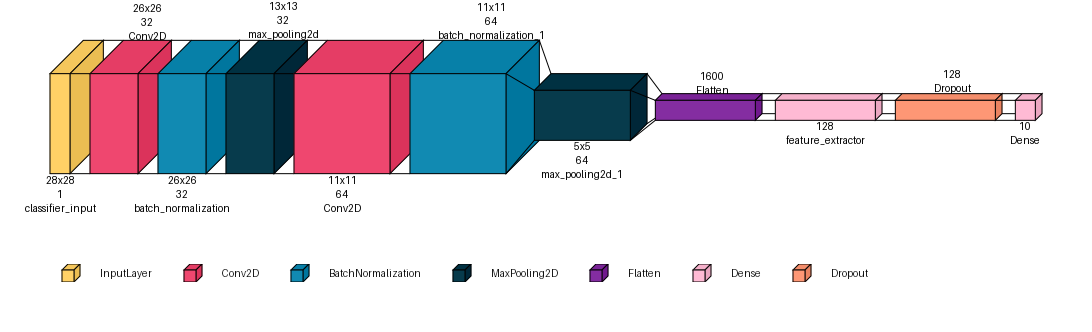
\includegraphics[width=.9\textwidth]{abb/netron_network_archs/classifying_Classifier_MNIST.png}
    \caption{Depiction of the CNN achritecture used to classify unlabeled images from the MNIST GDA experiments. (Image created with \cite{Gavrikov2020VisualKeras})}
    \label{fig:figure_class_mnist}
\end{figure}

\begin{figure}[htbp]
    \centering
    \vspace{-2em}
    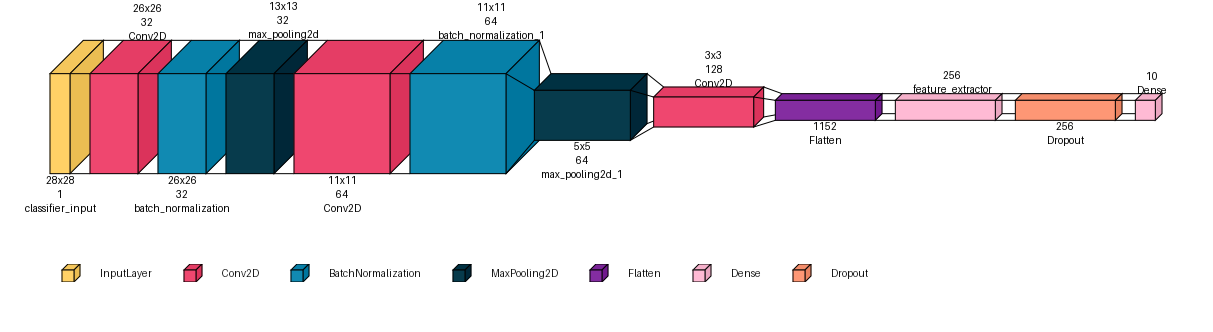
\includegraphics[width=.9\textwidth]{abb/netron_network_archs/classifying_Classifier_FashionMNIST.png}
    \caption{Depiction of the CNN achritecture used to classify unlabeled images from the FashionMNIST GDA experiments. (Image created with \cite{Gavrikov2020VisualKeras})}
    \label{fig:figure_class_fashion}
\end{figure}

\begin{figure}[htbp]
    \centering
    \vspace{-2em}
    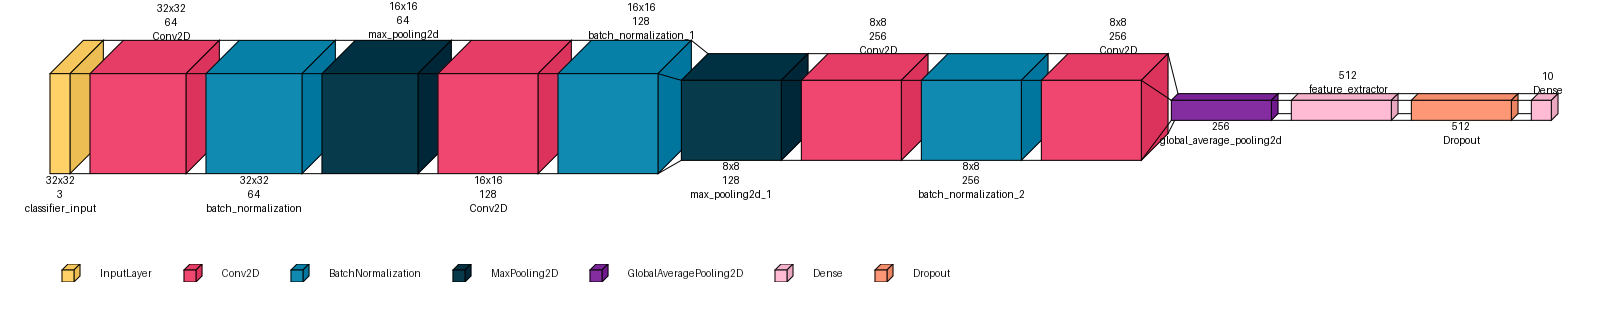
\includegraphics[width=.9\textwidth]{abb/netron_network_archs/classifying_Classifier_Cifar10.png}
    \caption{Depiction of the CNN achritecture used to classify unlabeled images from the CIFAR10 GDA experiments. (Image created with \cite{Gavrikov2020VisualKeras})}
    \label{fig:figure_class_cifar10}
\end{figure}

%Mention the classifiers trained and used to label the unlabeled data.

\subsection{Calculation of FID and IS}

asdfasdfasdfadfasdfasd 
%TODO: mention the experiments made with basing a calculation of these scores on self trained classifiers?




% EXPLAIN HOW THE FID AND IS SCORES ARE CALCULATED
% --> MENTION THAT EXPERIMENTS HAVE BEEN MADE TO USE SELF-TRAINED CLASSIFIERS/FREATURE-EXTRACTORS FOR THE MNIST AND FASHION DATASETS AND WHY THE DESCICION WAS MADE AGAINST THIS APPROACH -- SINCE ITS ONLY SELF-REFERENTIOAL AND SELF COMPARING, IT IS FINE TO USE THE INCEPTIONV3 MODEL FOR ALL DATASETS.

% EXPLAIN HOW THE DATA FOR EACH CLASSIFIER WAS GENERATED
% EXPLAIN THE CLASSIFIERS THEMSELVES
%
%##########################################

%##########################################
% How are the fid and is calculated?
% Explain for all three datasets
%##########################################








\newpage
